\chapter{Design and Implementation}

In this section...

\section{Data Collection}
We collected our own data for this research. Twitter has an Application Programming Interface (API) that allows developers to easily collect large quantities of tweets. The data was collected between October 2017 and September 2018.

All of the tweets collected were Geo-tagged. This means they all have location data, a specified location from which they were posted. There are two main types of Geo-tagged tweets:
\begin{itemize}
    \item Tweets with a specific latitude/longitude 'Point' coordinate. These tweets come from GPS enabled devices (Listing ~\ref{lst:pointjson}).
    \item Tweets with a bounding box or Twitter 'Place'. A bounding box is a four-sided geographic area, defined by four points in the form [longitude, latitude]. This defines the general area the tweet was posted from (Listing ~\ref{lst:placejson}).
\end{itemize}

Only 7.23\% of the tweets in our collection have a specific 'Point' coordinate. The rest have a Twitter 'Place' defining the general area the tweet was posted from.
\newline
\begin{lstlisting}[caption={Geo-tagged Tweet with Point Coordinate},captionpos=b,label=lst:pointjson,language=json,firstnumber=1]
"geo": {
    "type": "Point",
    "coordinates": 
        53.28581863,
        -6.11439315
    ]
}
\end{lstlisting}

\begin{lstlisting}[caption={Geo-tagged Tweet with Twitter Place},captionpos=b,label=lst:placejson,language=json,firstnumber=1]
"place": {
  "full_name": "Dun Laoghaire-Rathdown, Ireland",
  "url": "https://api.twitter.com/1.1/geo/id/723427e351a01e72.json",
  "country": "Ireland",
  "place_type": "city",
  "bounding_box": {
    "type": "Polygon",
    "coordinates": [
      [
        [
          -6.282038,
          53.199283
        ],
        [
          -6.282038,
          53.315283
        ],
        [
          -6.066759,
          53.315283
        ],
        [
          -6.066759,
          53.199283
        ]
      ]
    ]
  },
  "country_code": "IE",
  "attributes": {},
  "id": "723427e351a01e72",
  "name": "Dun Laoghaire-Rathdown"
}
\end{lstlisting}

The bounding box operator was used. This operator allows you to specify a bounding box from which all tweets collected must be posted from. A bounding box is a four-sided geographic area, defined by four points in the form [longitude, latitude]. Any tweet containing a 'Point' or 'Place' that falls fully within the specified bounding box is collected. 

Ethical considerations of collecting Twitter Data.

\section{Data Processing}

\subsection*{Extract Dublin Tweets}

The first thing that had to be done was to filter out any tweets that were not from Dublin. A bounding box for the Dublin area was defined (Table ~\ref{tab:dublinbb}). Tweets with a 'Point' coordinate and tweets with a Twitter 'Place' were treated differently:
\begin{itemize}
    \item Each tweet with a 'Point' coordinate was checked to see if it fell within the defined bounding box for Dublin, if it fell outside it was filtered out.
    \item Each tweet with a Twitter 'Place' has a bounding box specifying the 'Place'. The centroid of each tweets bounding box was calculated. Then the centroid was checked to see if it fell within the defined bounding box for Dublin, if it fell outside it was filtered out.
\end{itemize}

The centroid was calculated by...

\begin{table}[h!]
\caption{Coordinates for Dublin's Bounding Box}
\label{tab:dublinbb}
\begin{tabular}{|l|l|}
\hline
North Latitude  & 53.425210 \\ \hline
South Latitude  & 53.223430 \\ \hline
East Longitude & -6.043924 \\ \hline
West Longitude & -6.447485 \\ \hline
\end{tabular}
\end{table}

\subsection*{Extract Hotel Tweets}

\section{Dataset Annotation}

\subsection*{Webpage}

A simple webpage was created in order to annotate the tweets (Figure ~\ref{fig:webpage}. \newline
It can be found at \url{http://reviewtweets.epizy.com/}

\begin{figure}[h!]
\centering
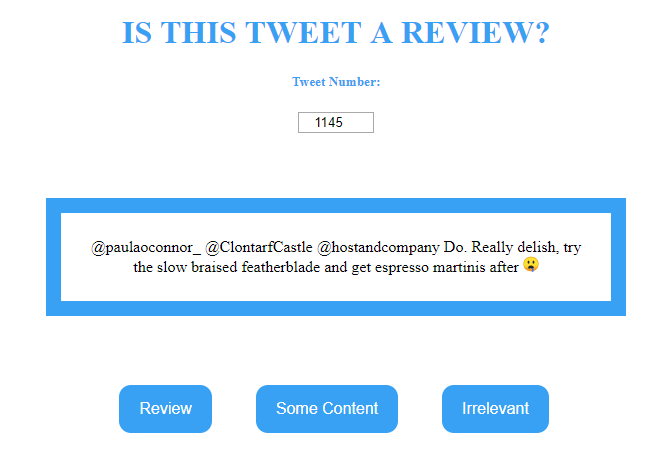
\includegraphics[width=1\textwidth]{project/webpage.PNG}
\caption{\label{fig:webpage} Webpage for gathering Tweet Annotations.}
\end{figure}

The following instructions accompanied the webpage:
\begin{itemize}
    \item \textbf{Review} \newline
    The tweet could be considered as a review (of any aspects related to a hotel such as the venue, food, view, swimming pool etc.) for any hotel. Examples would include: \emph{"Amazing view of the Aviva Stadium from my hotel balcony at hotel X"} (positive review), "Room service was awful at hotel Y" (negative review), \emph{"Thank you hotel X for a lovely stay"} (positive review) or \emph{"Had an awful night at hotel Y"} (negative review).
    \item \textbf{Some Content} \newline
    The tweet doesn't look like a review, but it does provide some information related to a hotel, such as the hotel hosts events, information on the menu, information related to accommodation etc. Examples would include: \emph{"Hotel Z serves Tuna salad on Wednesday”} or \emph{“A packed room for the 2018 fashion conference at Hotel X”}.
    \item \textbf{Irrelevant} \newline
    This tweet is completely irrelevant. While perhaps mentioning the name of a hotel, the tweet doesn't give any additional information about that hotel or offer any opinions related to the hotel.
\end{itemize}

For this research we decided to focus entirely on the text of the tweets. For this reason all images, videos and URLs were removed from the tweets.

The webpage was circulated and annotations were gathered.

\section{Tweet Classification}

\section{Sentiment Analysis}

Stanford NLP

\section{Recommender System}

CoRE
